\documentclass[border=10pt]{standalone}
\usepackage{pgfplots}
\pgfplotsset{compat=1.18}
\usepgfplotslibrary{colormaps}

\begin{document}
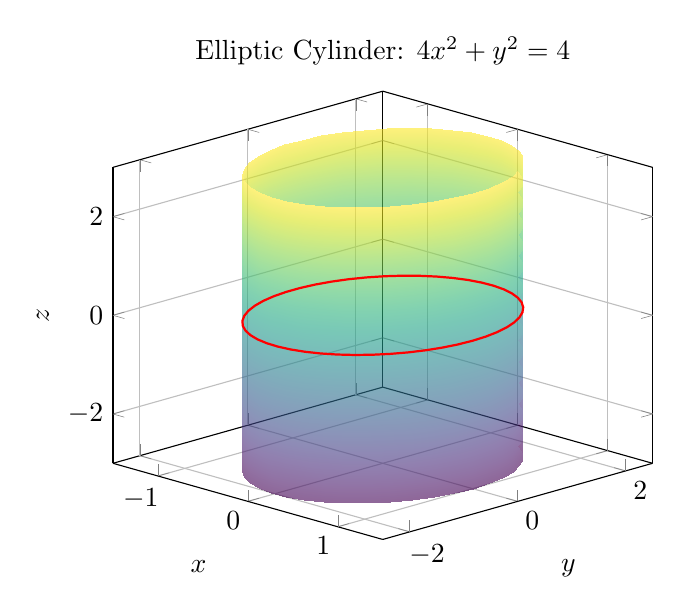
\begin{tikzpicture}
\begin{axis}[
    view={45}{20},
    xlabel={$x$},
    ylabel={$y$},
    zlabel={$z$},
    title={Elliptic Cylinder: $4x^2 + y^2 = 4$},
    grid=major,
    colormap/viridis,
    zmin=-3, zmax=3,
    xmin=-1.5, xmax=1.5,
    ymin=-2.5, ymax=2.5,
    ]
    
    % Plot the cylinder surface using parametric equations
    \addplot3[
        surf,
        shader=interp,
        opacity=0.6,
        domain=0:360,
        y domain=-3:3,
        samples=40,
        samples y=15,
    ]
    ({cos(x)}, {2*sin(x)}, {y});
    
    % Add reference ellipse at z=0
    \addplot3[
        domain=0:360,
        samples=50,
        thick,
        red,
    ]
    ({cos(x)}, {2*sin(x)}, 0);
    
\end{axis}
\end{tikzpicture}
\end{document}